\documentclass[10pt]{article}
\usepackage[a4paper,margin=25mm]{geometry}
\usepackage[T1]{fontenc}
\usepackage{lmodern,amsmath,amssymb,amsthm,booktabs,graphicx}
\usepackage{tikz,pgfplots}
\pgfplotsset{compat=1.18}
\usepackage[numbers,sort&compress]{natbib}
\usepackage[colorlinks=true,urlcolor=blue,citecolor=blue,linkcolor=blue]{hyperref}
\usepackage{microtype}
\newtheorem{theorem}{Theorem}
\newtheorem{lemma}[theorem]{Lemma}
\newtheorem{definition}[theorem]{Definition}
\newcommand{\R}{\mathbb R}
\newcommand{\Zn}{\mathbb Z/n\mathbb Z}
\newcommand{\supp}{\operatorname{supp}_{\rm cyc}}
\newcommand{\artifactdoi}{10.5281/zenodo.23474352}
\newcommand{\emptyartifactdoi}{} % Insert only the DOI actually reserved for this release.
\title{Terminal-Scalar-Aware Compilation of Quadratic Scores for CKKS}
\author{Leonard van Hemert}
\date{19 October 2026}
\begin{document}
\maketitle
\begin{abstract}
An encrypted scalar quadratic score need not preserve the intermediate matrix--vector product used to evaluate it. We study a compiler pass for public symmetric quadratic forms that chooses $A$ with $A+A^\top=2Q$ before applying existing CKKS linear-transform kernels. Orienting opposite cyclic offsets gives at most $\lfloor n/2\rfloor+1$ active diagonals in every positive dimension. We prove a matching lower bound among these representatives when every cyclic diagonal of $Q$ contains a nonzero entry. This is a support optimum, not a ciphertext-circuit or runtime optimum. The implementation uses pinned Lattigo kernels and compares symmetric, triangular, direct, BSGS, and additional quadratic baselines. In separate client/server processes at batch 128, selected plans reduce full loopback inference time by 4.6\%, 16.5\%, and 14.0\% at dimensions 8, 16, and 32, with lower measured server peak memory. A faster dimension-32 plan increases memory and evaluation-key requirements; a dimension-8 BSGS plan is slower. All use the same parameters, security assessment, model, and $10^{-3}$ absolute-error requirement. Exact rational correspondence checks, encrypted validation, frozen records, and a Lean project expose distinct mathematical, numerical, and implementation verification boundaries. Historical priority for this precise compiler rule remains unestablished.
\end{abstract}

\section{Problem and contribution}
Consider a public score
\begin{equation}\label{eq:score}
f(x)=x^\top Qx+\ell^\top x+c,\qquad Q=Q^\top\in\R^{n\times n}.
\end{equation}
The client encrypts $x$, the server computes on ciphertexts, and only the client decrypts the final score. The target includes square-activation neural scores
\[
a\left(\sum_{k=1}^{h}v_k(w_k^\top x+b_k)^2+c_{\rm out}\right),
\]
whose public coefficients can be folded exactly to \eqref{eq:score}. Folding alone is an essential baseline, not the proposed contribution. The measured domain is $[-1,1]^n$, $n\in\{8,16,32\}$, with 128 independent examples per encrypted request. The construction is general in positive dimension; this particular Go packing/backend supports power-of-two dimensions and the measured dimensions are 8, 16, and 32. The algebraic theorem and Python construction are not restricted to powers of two. We do not claim classifier accuracy on a trained application, a general deep-network speedup, or improved bootstrapping.

A conventional lowering computes $Qx$, multiplies componentwise by $x$, and sums. When that vector has no other consumer, it suffices to preserve its scalar contraction. The pass studied here selects $A$ satisfying
\begin{equation}\label{eq:admissible}
A+A^\top=2Q
\end{equation}
and computes $\sum_i x_i((Ax)_i+\ell_i)+c$. This enlarges the compiler's choice before lowering to existing kernels. A triangular representative already exploits symmetry, but ordinary index-order triangularity can leave every cyclic diagonal active. Orienting \emph{offset pairs}, rather than individual index-ordered pairs, exposes a different sparse linear transform.

The candidate contribution comprises a precise scalar-consumer rewrite, a general restricted support theorem, an implementation correspondence check, and measured interaction with CKKS plans and lifecycle costs. Elementary quadratic identities, skew-symmetric freedom, triangular elimination, diagonal decompositions, BSGS, hoisting, and cryptographic constructions are not claimed as inventions. Nor does the absence of a located matching paper establish historical priority. The release makes a useful mechanism independently inspectable without requiring a priority claim.

\section{Threat model and requirements}\label{sec:threat}
One client owns the secret key, inputs, and final outputs. The server is honest but curious: it follows the prescribed computation and attempts to infer information from its observations. Model weights, dimensions, batch size, parameters, schedule, timing, memory use, evaluation keys, and serialized lengths are public. The client sends no decrypted intermediate values, decoded outputs, error statistics, or acceptance decisions to the server. Client packing only replicates coordinates; it performs no model-dependent feature extraction. The synthetic benchmark fixtures are deliberately public research evidence, rather than private deployment inputs.

The principal measurement uses distinct processes. The server is an exec-child launched before client keys and fixtures are initialized, receives sanitized public configuration through a pipe, and receives evaluation keys and encrypted requests over HTTP. Its interface has no secret-key/decryptor argument. The client alone decrypts the returned final ciphertext. This process separation is an architectural check, not an alternative cryptographic assumption. Older combined-role experiments are explicitly identified in Section~\ref{sec:secondary}.

The security target is classical Category 128 under the selected CKKS/RLWE assumptions, assessed using published parameter guidance. We claim neither a new cryptographic proof nor a fresh lattice-estimator run. Passive privacy does not supply malicious-server integrity or circuit privacy; no decryption-feedback protocol is introduced. Every compared method must meet the same $10^{-3}$ absolute-error threshold against the original neural score, with unchanged model coefficients, no rank truncation, retraining, or activation approximation. Exact algebra and observed CKKS error are assessed separately.

\section{Construction and complete support proof}\label{sec:math}
Index rows and columns by $\Zn$, where $n>0$, and let $\bar r\in\{0,\ldots,n-1\}$ denote the canonical integer representative. Define
\[
S(M)=\supp(M)=\{r\in\Zn:\exists i,\ M_{i,i+r}\ne0\}.
\]
A representative is \emph{admissible} for $Q$ when \eqref{eq:admissible} holds. Call $Q$ \emph{cyclically dense} if for every $r\in\Zn$ there is at least one $i$ with $Q_{i,i+r}\ne0$. This is weaker than requiring every entry nonzero, but stronger than requiring some off-diagonal entries nonzero. It is the explicit hypothesis for the lower bound.

\begin{theorem}[Scalar preservation]\label{thm:preserve}
For real matrices $Q,A$ of equal finite dimension, if $A+A^\top=2Q$, then $x^\top Ax=x^\top Qx$ for every real vector $x$. Hence the affine quadratic scores with the same $\ell,c$ agree everywhere.
\end{theorem}
\begin{proof}
Let $q_M(x)=\sum_{i,j}x_iM_{ij}x_j$. Exchanging the finite indices $i,j$ and using commutativity gives $q_{A^\top}(x)=q_A(x)$. Multiplying the entrywise hypothesis by $x_ix_j$ and summing gives
$2q_A(x)=q_A(x)+q_{A^\top}(x)=2q_Q(x)$. Division by $2$ in $\R$ proves the claim. Adding the identical affine terms preserves equality. Symmetry of $Q$ is unnecessary for this implication (and follows from the existence of an admissible $A$).
\end{proof}

Let $C_n=\{r:\bar r\le\overline{-r}\}$. The \emph{cyclic orientation} of symmetric $Q$ is
\begin{equation}\label{eq:orientation}
O(Q)_{ij}=\begin{cases}
Q_{ij},&r=-r,\\
2Q_{ij},&\bar r<\overline{-r},\\
0,&\bar r>\overline{-r},
\end{cases}\qquad r=j-i\in\Zn.
\end{equation}
The self-inverse offsets are $0$ and, when $n$ is even, $n/2$. They are retained without doubling. Thus $C_n$ consists of offsets $0$ through $\lfloor n/2\rfloor$. This also specifies the cases $n=1$ and $n=2$ without exception.

\begin{theorem}[Orientation preservation and support]\label{thm:upper}
For every $n>0$ and symmetric $Q$, $O(Q)+O(Q)^\top=2Q$, so the score is preserved for every $x$. Moreover,
\[
S(O(Q))\subseteq C_n,\qquad |S(O(Q))|\le\lfloor n/2\rfloor+1.
\]
\end{theorem}
\begin{proof}
For a fixed pair $(i,j)$ the transposed entry has offset $-r$. If $r=-r$, both oriented entries equal their symmetric $Q$ entries and sum to $2Q_{ij}$. Otherwise exactly one of $\bar r<\overline{-r}$ and its reverse holds. The two entries are therefore $2Q_{ij}$ and $0$, whose sum is again $2Q_{ij}$. Theorem~\ref{thm:preserve} applies. Entries outside $C_n$ vanish by definition. For nonzero $r$, $\overline{-r}=n-\bar r$, so membership in $C_n$ is exactly $2\bar r\le n$; the zero offset also belongs. There are $\lfloor n/2\rfloor+1$ such integers. This proves the support bound in odd, even, and singleton dimensions.
\end{proof}

\begin{theorem}[Matching restricted lower bound]\label{thm:lower}
Let $n>0$ and let $Q$ be cyclically dense. Every admissible $A$ satisfies
\[
|S(A)|\ge\lfloor n/2\rfloor+1.
\]
Consequently, when $Q$ is also symmetric, the orientation attains the minimum cyclic-support cardinality among all admissible representatives.
\end{theorem}
\begin{proof}
For each $r$ choose $i$ with $Q_{i,i+r}\ne0$. Admissibility gives
$A_{i,i+r}+A_{i+r,i}=2Q_{i,i+r}\ne0$, so at least one of $r,-r$ lies in $S=S(A)$. Thus $S\cup(-S)=\Zn$. For $r=0$ the same argument forces $0\in S$, hence $0\in S\cap(-S)$. Negation is a bijection, so
\[
n=|S\cup(-S)|=2|S|-|S\cap(-S)|\le2|S|-1.
\]
It follows that $|S|\ge\lceil(n+1)/2\rceil=\lfloor n/2\rfloor+1$. In even dimensions the self-inverse half-turn is itself forced into $S$; the displayed weaker intersection estimate already yields the required integer bound. The upper bound in Theorem~\ref{thm:upper} matches it. The argument does not hypothesize a lower bound on support and does not restrict $A$ to the particular orientation algorithm.
\end{proof}

The theorem concerns a matrix representation lowered through cyclic diagonals. It does not lower-bound rotations after BSGS, temporary memory, key-switch cost, or arbitrary encrypted circuits. For sparse $Q$, cyclic density can fail and the stated lower bound need not apply. An implementation should omit exact zero diagonals and compare the original plan as well as the oriented plan.

\paragraph{Compiler rule.}
The sole-consumer check is a semantic precondition: rewriting $Qx$ would be invalid if another consumer needed that vector. Public folding and admissibility checks precede encrypted execution. A deterministic rule is:
\begin{quote}\small\ttfamily
Require a terminal real scalar sum(i, x[i] * y[i]);\\
fold public quadratic coefficients into symmetric Q, ell, c;\\
for every i,j: r = (j-i) mod n;\\
\hspace*{1em}if r == -r: A[i,j] = Q[i,j];\\
\hspace*{1em}else if value(r) < value(-r): A[i,j] = 2*Q[i,j];\\
\hspace*{1em}else: A[i,j] = 0;\\
check exact A + transpose(A) == 2*Q;\\
lower A using candidate direct/BSGS plans;\\
retain baseline if the deployment objective prefers it.
\end{quote}
The Python API rejects nonsymmetric, nonfinite, nonsquare, or overflowing inputs. Its postcondition is checked using exact rational interpretations of stored binary64 numbers. For the frozen dyadic models, public folding has zero coefficient residual. Arbitrary public inputs may have a reported storage residual and must satisfy the same error budget.

\section{CKKS realization and deployment cost}\label{sec:ckks}
We use CKKS~\citep{ckks} through Lattigo v6.2.0~\citep{lattigo}. Standard CKKS at ring degree $N=8192$ has 4096 complex slots. For batch $B=128$, feature $i$ of example $b$ is placed in slot $iB+b$, repeated with period $nB$ across all slots. Since $nB$ divides 4096 in the measured dimensions, a rotation by $rB$ implements a cyclic feature shift without mixing examples. The client performs replication only. Matrices $Q$, triangular representatives, and oriented representatives use this identical layout, encrypted input size, and output size.

The server forms $Ax$ using diagonal plaintexts and the official hoisted direct or BSGS linear-transform evaluator, rescales, and adds $\ell$. It drops one level of the unchanged encrypted $x$, multiplies it componentwise with $Ax+\ell$, relinearizes, rescales, and reduces the $n$ feature blocks using $\log_2n$ rotations. Adding $c$ finishes the score. Only the resulting ciphertext returns to the client. Both baseline and candidate use one ciphertext--ciphertext multiplication, one relinearization, two rescale levels, and zero bootstraps. The multiplicative depth in variable--variable products is one; two consumed rescale levels should not be confused with two such products.

For a dense model, orientation changes the plaintext diagonal-product count from $n$ to $n/2+1$ in the measured even dimensions. It does not reduce ciphertext multiplication depth. Direct lowering generally eliminates input rotations and keys; BSGS can change this relationship because its baby/giant grouping and key set depend on the support. Kernel scheduling and hoisting remain existing backend mechanisms~\citep{halevishoup}. A support-optimal matrix need not give the fastest or smallest-memory plan.

\paragraph{Parameters.}
The final Standard configuration uses $\log_2 Q_i$ bit sizes $[58,40,40]$, auxiliary modulus bit size $[60]$, scale $2^{40}$, uniform ternary secret, and default truncated Gaussian error with $\sigma=3.2$. The actual primes are
\begin{align*}
Q&=[288230376151760897,1099511480321,1099511922689],\\
P&=[1152921504606830593].
\end{align*}
Their measured $\log_2(QP)\approx198.0000002$, including the key-switching auxiliary prime. Prime/congruence checks and modulus-bit accounting are part of the evidence validation. The assessment compares this with the published uniform-ternary $N=8192$ Category-128 bound of 214 bits~\citep{securityguidelines}. This is a published-table assessment under stated assumptions, not a security proof or an unperformed estimator computation. Earlier development used $P=50$; those smoke results are separate, and final comparisons share $P=60$. The final modulus-to-scale ratio is about $2^{18}$; the archived model's global score bound of 1814 lies within its centered range. The main evidence here uses Standard CKKS. Conjugate-invariant comparisons are secondary matched-batch experiments with their separate ring assumptions; their extra slot capacity is not silently assigned to the candidate.

\paragraph{Lifecycle objective.}
For a client key reused over $H$ inferences, choose among measured legal plans using
\begin{equation}\label{eq:lifecycle}
F+S_p+HT_p,\qquad K_p\le K_{\max},\quad M_p\le M_{\max}.
\end{equation}
Here $F$ is once-per-public-model folding, $S_p$ includes public encoding, key generation/serialization, key distribution and installation, startup and warmup, and $T_p$ is the complete recurring encrypted chain. $K_p$ is serialized evaluation-key size and $M_p$ is peak server RSS. The implementation's profile-based selector is an explicit optimization over candidates, not a request for an LLM to guess cryptographic parameters. Memory and key constraints can choose dimension-32 BSGS over faster direct execution.

Measured HTTP distribution is loopback TCP. For WAN planning one can explicitly add bandwidth and latency estimates to \eqref{eq:lifecycle}, using key and ciphertext byte counts. Such a model is not a measured WAN result; do not double-count measured loopback transport. Setup is neither omitted nor folded into per-inference time without a stated $H$.

\section{Correctness, error, and formal verification}\label{sec:verification}
Theorems~\ref{thm:preserve}--\ref{thm:lower} are exact statements over the reals. Public folding, stored coefficients, and CKKS execution introduce separate obligations. For a residual polynomial $x^\top Rx+s^\top x+t$ and $\|x\|_\infty\le R_0$,
\begin{equation}\label{eq:residual}
|x^\top Rx+s^\top x+t|\le R_0^2\sum_{ij}|R_{ij}|+R_0\sum_i|s_i|+|t|.
\end{equation}
This follows term by term from the triangle inequality. The exact rational checker uses this bound for coefficient certificates, including affine square comparators. It does not discard small eigenvalues. For orientation the stored-coefficient residual is exactly zero in the frozen models.

If an input perturbation has $\|e\|_\infty\le\eta$, direct expansion yields
\[
|f(x+e)-f(x)|\le(2R_0\eta+\eta^2)\sum_{ij}|Q_{ij}|+\eta\|\ell\|_1.
\]
For symmetric $Q$, orientation preserves the total entrywise coefficient mass: every non-self-inverse pair replaces two equal-magnitude entries by one doubled entry, and self-inverse entries are unchanged. Thus it does not increase this particular global mass bound. This fact is insufficient to bound CKKS error: different key-switching and accumulation schedules still have different numerical behavior.

A conditional execution bound would propagate proven linear-transform, rescale, product, and reduction error bounds. For example, for $g_i=(Ax)_i+\ell_i$,
\[
|(x_i+e_i)(g_i+d_i)-x_ig_i|
\le |x_i||d_i|+|g_i||e_i|+|e_i||d_i|.
\]
Such intermediate CKKS bounds have not been proved uniformly on the box here. The release therefore reports empirical encrypted errors, not a domain-wide noise theorem or a statistical independence claim.

\paragraph{Lean boundary.}
The release contains a pinned Lean 4/mathlib project. Its checked principal declarations, in namespace \texttt{FHEQuadratic}, map directly to the mathematical statements:
\begin{center}\small
\begin{tabular}{ll}\toprule
Paper claim & Lean declaration\\\midrule
Theorem~\ref{thm:preserve} & \texttt{quadratic\_preservation}\\
Affine extension & \texttt{affine\_score\_preservation}\\
Orientation admissibility & \texttt{orientation\_admissible}\\
Orientation score equality & \texttt{orientation\_preservation}\\
$|C_n|=\lfloor n/2\rfloor+1$ & \texttt{canonicalOffsets\_card}\\
Theorem~\ref{thm:upper}, support bound & \texttt{orientation\_support\_upper\_bound}\\
Theorem~\ref{thm:lower}, lower bound & \texttt{activeOffsets\_card\_lower\_bound}\\
Attainment and optimality & \texttt{orientation\_support\_exact},\\
& \texttt{orientation\_support\_optimal}\\\bottomrule
\end{tabular}
\end{center}
The integrated \texttt{lake build} passed on 19 October 2026 with Lean 4.24.0 and mathlib v4.24.0 (the exact revision is pinned in the dependency lock). The actual axiom-dependency checker passed for all eleven principal declarations: each printed dependency set is exactly \texttt{[propext, Classical.choice, Quot.sound]}. These are standard logical axioms; no additional mathematical axiom, \texttt{sorryAx}, admitted goal, or kernel-bypass mechanism is used. Exact commands, versions, build results and \texttt{\#print axioms} output are documented in \path{docs/FORMAL_VERIFICATION.md}.

\texttt{scripts/check\_correspondence.py} checks exported matrices using exact rational arithmetic, independently of encrypted timings: 41 matrices and seven public network folds are checked in the release evidence. It connects implementation outputs on those fixtures with the defined orientation formula and admissibility equation, not every future program execution. Formal algebra does not verify the Go evaluator, cryptographic security, compiler/runtime implementation, hardware measurements, or uniform numerical noise. These exclusions remain even after Lean succeeds.

\section{Experimental evidence}\label{sec:experiments}
All historical timing records use an Apple M4 MacBook Air, 16 GiB RAM, Darwin arm64, Go 1.25.3 and Lattigo v6.2.0. The execution thread setting is \texttt{GOMAXPROCS=1}; the principal separate-process arm has one Go execution thread per role. Batch, parameters, layout, coefficient model, error requirement and hardware are matched within each comparison. Frozen model labels contain seed numbers such as 20261020; those numbers are reproducibility seeds, not claims of later measurement dates.

Seven models were predetermined in \texttt{artifacts/models.json}: an archived integer dimension-8/64-hidden-unit model, synthetic dimension-8/64, dimension-16/128 and dimension-32/128 indefinite scores, held-out dimension-8/96 and dimension-16/96 seeds, and a dimension-16/64 positive-definite score. Synthetic normalization was fixed before benchmarking and applied equally to all methods. Held-out model seeds were not used to choose the mechanism or parameters.

The broad portfolio includes the original packed square network, fused symmetric and ordinary triangular quadratic contraction, direct and official BSGS settings, spectral/LDL affine squares, feature-layout alternatives, and a real conjugate-invariant arm. It contains 336 final model/method records. The fastest tested complete codec-chain baseline is selected per model; this is stronger than comparing with an unfused or untuned network alone. It remains a finite tested portfolio, not proof that every existing implementation has been optimized or outperformed. No complete Orion, HEIR, or other compiler suite was reproduced.

\subsection{Principal separate-process measurements}\label{sec:primary}
Table~\ref{tab:main} comes from five counterbalanced fresh process/key rounds with 31 timed fresh encryptions per plan after separately charged warmup. Each timing is the median of five process medians. RSS is the median of the server child's maximum resident-set value from exit resource usage, not a summed client/server peak. Keys and RSS use decimal MB. The chain includes packing/encoding, encryption, ciphertext serialization, loopback request, server evaluation, response, deserialization and final client decryption/decoding. Evidence-file writes and plaintext reference validation are outside timing.

\begin{table}[t]
\centering\small
\resizebox{\linewidth}{!}{\begin{tabular}{rlrrrrr}
\toprule
$d$ & Plan & Server ms & Chain ms & RSS MB & Keys MB & Setup ms \\
\midrule
8 & triangular\_direct & 6.188 & 8.715 & 86.98 & 12.586 & 68.99 \\
8 & oriented\_direct & 5.541 & 8.310 & 65.77 & 7.866 & 53.19 \\
8 & oriented\_bsgs3 & 6.854 & 9.427 & 59.79 & 7.866 & 52.11 \\
16 & triangular\_direct & 9.429 & 12.139 & 127.22 & 25.172 & 110.61 \\
16 & oriented\_direct & 7.413 & 10.139 & 90.36 & 14.159 & 72.27 \\
16 & oriented\_bsgs3 & 8.713 & 11.547 & 82.49 & 14.159 & 74.51 \\
32 & symmetric\_bsgs3 & 16.174 & 19.983 & 105.43 & 17.306 & 171.58 \\
32 & oriented\_direct & 11.937 & 15.597 & 135.09 & 26.745 & 159.95 \\
32 & oriented\_bsgs3 & 13.502 & 17.181 & 85.98 & 15.732 & 118.79 \\
\bottomrule
\end{tabular}
}
\caption{Actual separate client/server processes, $B=128$. Setup is charged separately from the recurring chain. All plans use identical final parameters and quality requirements.}\label{tab:main}
\end{table}

Using ratios of the displayed marginal medians, dimension-8 oriented direct reduces chain time by 4.6\%, server RSS by 24.4\%, and keys by 37.5\%; dimension-16 oriented direct reduces them by 16.5\%, 29.0\%, and 43.8\%. Dimension-32 oriented BSGS3 reduces them by 14.0\%, 18.4\%, and 9.1\%. These percentages must not be read as paired-round estimates. Paired chain speedup medians are respectively 1.086, 1.207 and 1.148, with ranges 1.029--1.154, 1.180--1.228 and 1.006--1.175; each selected plan wins all five paired rounds. The median-of-ratios aggregation need not equal the ratio of marginal medians; round-level timing drift may affect either. Five rounds do not establish a hardware-independent performance distribution.

Figure~\ref{fig:tradeoffs} preserves unfavorable results. Dimension-8 BSGS3 is slower on the aggregate chain despite its smaller RSS. Dimension-32 direct is fastest, but its RSS is 135.09 rather than 105.43 MB and its keys are 26.745 rather than 17.306 MB. It is therefore unsuitable as a claimed memory win. The memory-constrained BSGS plan is a different point on the tradeoff curve.

\begin{figure}[t]\centering
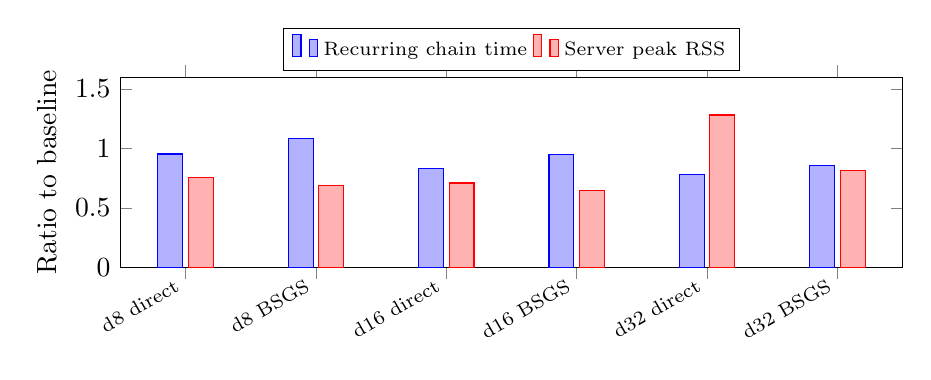
\begin{tikzpicture}
\begin{axis}[ybar,bar width=9pt,width=0.95\linewidth,height=4cm,ylabel={Ratio to baseline},symbolic x coords={d8 direct,d8 BSGS,d16 direct,d16 BSGS,d32 direct,d32 BSGS},xtick=data,x tick label style={rotate=30,anchor=east,font=\scriptsize},ymin=0,ymax=1.6,legend style={font=\scriptsize,at={(0.5,1.03)},anchor=south,legend columns=2}]
\addplot coordinates {(d8 direct,0.95355016) (d8 BSGS,1.08173564) (d16 direct,0.83524869) (d16 BSGS,0.95122373) (d32 direct,0.78052946) (d32 BSGS,0.85977906)};
\addlegendentry{Recurring chain time}
\addplot coordinates {(d8 direct,0.75607459) (d8 BSGS,0.68732341) (d16 direct,0.71023825) (d16 BSGS,0.64842241) (d32 direct,1.28127428) (d32 BSGS,0.81554002)};
\addlegendentry{Server peak RSS}
\end{axis}
\end{tikzpicture}

\caption{Separate-process marginal-median ratios from raw records. Lower is better. Reducing diagonal support is not a universal time or memory improvement.}\label{fig:tradeoffs}
\end{figure}

Operation records explain rather than replace measurements. At $n=8$, direct orientation changes diagonal products from eight to five and total logical rotations from ten to seven; the distinct rotation-key count changes from seven to four. At $n=16$ the corresponding counts are 16 to nine, 19 to 12, and 15 to eight. The reduction rotations remain charged. At $n=32$ BSGS schedule structure matters: a smaller diagonal set alone does not predict the key or temporary-memory cost. Every matched packed plan still has one ciphertext product, one relinearization, two rescale levels, and zero bootstraps.

Separate-process setup includes parent public encoding, child startup and configuration transfer, child public encoding, key generation/serialization, HTTP installation, warmup, and child shutdown. The redundant parent/child encoding is charged. Embedded key-deserialization time is not added to its enclosing round-trip twice. Network-to-quadratic folding is separately once-per-public-model. Under this measured loopback lifecycle, both dimension-32 candidates amortize against the baseline at $H=1$; BSGS3 has lower setup and recurring time. This does not imply the same threshold on a WAN.

\subsection{Broader and combined-role evidence}\label{sec:secondary}
Table~\ref{tab:sweep} reports the seven-model same-machine sweep with nine fresh encryptions after one warmup. Modes ran serially, so it is a breadth/ablation result and not the primary counterbalanced timing estimate. All rows use matched batch 128. The held-out seeds support generalization within this small scalar-quadratic class, not to arbitrary neural workloads.
\begin{table}[t]\centering\scriptsize
\resizebox{\linewidth}{!}{\begin{tabular}{llrrr}
\toprule
Model & Baseline & Base ms & Cand. ms & Speedup \\
\midrule
Archive 8/64 & packed/triangular\_direct & 6.370 & 5.836 & 1.091 \\
Development 8/64 & packed/triangular\_direct & 6.310 & 5.704 & 1.106 \\
Development 16/128 & packed/triangular\_direct & 7.844 & 6.813 & 1.151 \\
Development 32/128 & packed/symmetric\_bsgs3 & 10.621 & 8.460 & 1.255 \\
Held-out 8/96 & packed/symmetric\_direct & 6.130 & 5.652 & 1.085 \\
Held-out 16/96 & packed/symmetric\_bsgs3 & 9.303 & 8.084 & 1.151 \\
SPD 16/64 & packed/symmetric\_bsgs3 & 8.823 & 8.311 & 1.062 \\
\bottomrule
\end{tabular}
}
\caption{Broad matched-batch portfolio: fastest tested baseline per frozen model. These are combined-role measurements and must not be mixed with Table~\ref{tab:main}.}\label{tab:sweep}
\end{table}

A separate older combined-role HTTP confirmation contains five counterbalanced fresh processes per plan, 31 timed iterations, and actual loopback key/request transport. Its RSS includes client and server in one address space, unlike Table~\ref{tab:main}. It gives dimension-8 and -16 direct chain reductions of 9.3\% and 17.3\%; dimension-32 direct gives 19.7\% lower chain time but 35.3\% higher peak RSS. In that architecture its larger setup amortizes only at $H=7$, while dimension-32 BSGS3 wins from $H=1$. These results are retained as controlled ablations, not substituted for isolated server memory or compared in absolute time against the later separated runs. The complete generated table and raw records remain in the artifact.

\subsection{Numerical validation and integrity}
All 336 final portfolio records pass the fixed $10^{-3}$ absolute threshold; the worst portfolio error is $1.062\times10^{-5}$ in the conjugate-invariant archived-model arm. Reserved validation adds 560 encrypted batches using 40 fresh key/input seeds per model/method, with 49,000 uniform dyadic input--model pairs and boundary probes. Dimension 8 includes all 256 box corners, and signed basis and fixed boundary patterns are also checked. The maximum observed reserved-input absolute error is $4.24394575\times10^{-6}$. In the principal separate-process runs the maximum is $7.345\times10^{-8}$.

Vectors are reused across same-dimensional models, and outputs within a batch share keys. These are empirical zero-failure statements, not independent pooled trials or a uniform-box theorem. Plaintext neural references and exact coefficient certificates are separately checked. Historical ciphertexts are genuine serialized outputs, but secret keys are not persisted; fresh reruns perform full encryption/decryption rather than pretending the archived ciphertexts can be independently decrypted without those keys.

The release validator reads 685 run records, 986 method records, 2263 serialized ciphertexts and 249088 fixture outputs; these overlapping bookkeeping counts are not additional independent validation trials. It recomputes file integrity and aggregate evidence. Its clean-release checks are recorded separately from the original Apple M4 measurement campaign. Benchmark reruns write new directories and never overwrite the historical measurements. Generated tables and Figure~\ref{fig:tradeoffs} are committed outputs of \texttt{scripts/generate\_paper\_data.py}, and \texttt{--check} detects drift.

\section{Comparison with prior mechanisms}\label{sec:related}
The closest mathematical comparator is ordinary triangular symmetry elimination. Both choose a scalar-equivalent representative, but the orientation uses the cyclic-offset involution rather than linear index order; this distinction matters to a diagonal evaluator. Fused symmetric contraction is another necessary comparator: network folding can already remove many hidden squares. For the archived model, a separate inertia argument gives a minimum of $\max(p,m)=5$ products of real linear forms, since the inertia is $(3,5)$. To justify the general statement, if $q=\sum_{k=1}^t L_kR_k$, the common kernel of the $L_k$ has codimension at most $t$ and $q$ vanishes there. It intersects a positive-definite subspace or a negative-definite subspace only at zero, so $t\ge p,m$. Conversely, diagonalize the real symmetric form, pair positive and negative squares using $u^2-v^2=(u+v)(u-v)$, and leave any unmatched square as one product. This gives $t=\max(p,m)$. This algebraic cost model makes additions and public transforms free. It is not a 64/5 FHE speedup: at batch 128 the original 64 hidden squares occupy two ciphertexts, while fused contraction has one ciphertext product. Spectral/LDL and complex feature alternatives were executed and retained, but did not dominate the oriented packed plan at the primary workload.

Halevi--Shoup optimize homomorphic linear transforms with diagonal/BSGS and key-switching techniques~\citep{halevishoup}. We reuse existing kernels and change their input representative under scalar semantics. Coyote~\citep{coyote}, Fhelipe~\citep{fhelipe} and HECO~\citep{heco} already establish encrypted vectorization, layout selection and compiler restructuring; our work does not invent joint compilation. Orion~\citep{orion} supplies neural inference packing and scale/bootstrap planning, and HEIR~\citep{heir} provides a general integration framework. This prototype is not an implemented integration into either system and does not claim a cross-system benchmark win.

Equivalent-expression optimization also predates this work. Q-gym~\citep{qgym} exploits weight repetition through equality saturation. The specific pass here uses a closed-form representative construction and a terminal scalar's equivalence class. nGraph-HE2~\citep{ngraphhe2} provides complex packing and CKKS scheduling optimizations; client-assisted activation variants are outside the present no-intermediate-decryption protocol. These comparisons locate the candidate mechanism more precisely than claiming generic consumer-aware optimization is new.

KeyMemRT~\citep{keymemrt} is verified prior work with compiler/runtime implementations for rotation-key lifetime management, loading, clearing and prefetch. Eliminating some keys by changing the computation is distinct from managing an unchanged key set, and can coexist with that work. FHE-Agent~\citep{fheagent} is a verified Orion-based configuration preprint using an LLM controller. Its reported FHE runtime excludes key generation and its baseline is best-of-ten one-shot configurations; those author claims were not reproduced here. No official implementation was identified in the inspected manuscript, which is a bounded search observation. The present deterministic rewrite and measured lifecycle objective do not rely on an LLM choosing unexplained settings.

The bibliography and \texttt{docs/RELATED\_WORK.md} record primary-source metadata and implementation links. Our focused search has not established historical priority for the precise cyclic terminal-scalar pass. Publication acceptance, external peer review, or a broad breakthrough are not asserted.

\section{Reproducibility and limitations}
The release includes the Go backend and dependency lock, Python compiler/checkers, frozen models, measurements, generated material, integrity manifests, and the Lean toolchain/dependency locks. From the repository root, evidence-only checks include:
\begin{quote}\small\ttfamily
python3 scripts/check\_correspondence.py --check\\
python3 scripts/verify\_evidence.py --strict-ciphertexts\\
python3 scripts/generate\_paper\_data.py --check\\
cd lean \&\& lake build
\end{quote}
The complete clean-checkout instructions, encrypted rerun command, hardware qualifications and LaTeX build are in \texttt{REPRODUCING.md}. A rerun on different hardware establishes functioning encryption and accuracy, not reproduction of Apple M4 timing. Historical absolute paths inside raw command records are provenance; supported reproduction commands use the release checkout. Paper/data are licensed CC BY 4.0, and owned code/Lean files MIT; dependencies retain their own licenses.

The measured class is small exact public scalar quadratics with terminal consumers and favorable periodic packing. Multiple outputs, intervening nonlinearities, arbitrary dimensions/batches, and other architectures require separate evaluation. Sparse matrices can invalidate the dense-case optimality hypothesis. The selected plan depends on setup horizon, bandwidth, key memory and runtime memory; support minimization cannot replace profiling. The strongest supported result is an exact, restrictedly optimal representation pass with reproducible encrypted gains and explicit unfavorable cases. Empirical accuracy and published-table security assessment remain the stated evidence levels.

\ifx\artifactdoi\emptyartifactdoi\else
\paragraph{Artifact identifier.} \href{https://doi.org/\artifactdoi}{\texttt{\artifactdoi}}. The public release record, exact tag/commit and file hashes identify the archived version; DOI reservation alone is not publication.
\fi
\bibliographystyle{plainnat}
\bibliography{references}
\end{document}
